%!TEX root = ../CallenThermo.tex
% 翻译:SI
% 校对:lh

\chapter{Maxwell关系}
\label{chap7}

\section{Maxwell关系}
\label{sec7.1}
\ref{sec3.9}节\mpar{原文为\ref{sec3.6}节,根据内容来看应该是\ref{sec3.9}节。这里进行了修改。}讨论了绝热压缩率、热膨胀系数、摩尔热容等热力学量的物理意义。它们都具有$(\partial X / \partial Y)_{Z, W}$的形式,式中字母表示热力学广延量或强度量。一般的热力学系统有许多热力学量,从而可以构造大量这样的导数。但是众多的导数量之间存在羁绊,由此其中只有一小部分是独立的,其余的量可以用这一小部分表示。自然,这些关系可以大大简化热力学分析。并且我们不需要特意记忆公式\mpar{比如“{\bf G}ood {\bf P}hysicists {\bf H}ave {\bf S}tudied {\bf U}nder {\bf V}ery {\bf F}ine {\bf T}eachers”什么的……\sout{来自热统课的惨痛回忆}\ \sout{\ref{sec7.2}节有类似的另一句话} }。 下面介绍在热力学计算过程中用到的简单、直接推导这些关系的方法,也就是本章的主题。

首先说明这些导数量之间“羁绊”的存在性,考虑\eqref{equ3.70}与\eqref{equ3.71}式:
\begin{align}
	\frac{\partial^2 U}{\partial S \partial V} &= \frac{\partial^2 U}{\partial V \partial S}, \label{equ7.1} \\
	-\left( \frac{\partial P}{\partial S} \right)_{V, N_1, N_2} &= \left( \frac{\partial T}{\partial V} \right)_{S, N_1, N_2}. \label{equ7.2}
\end{align}
上式是导数量的“羁绊”——称为{\it Maxwell 关系 (Maxwell relations)}——的源头,亦即,导数量之间的依赖关系源自基本方程(在不同表象下)的混合导数不依赖于求导次序。

某一热力学量依赖于$(t + 1)$个自变量,从而有$t(t + 1)/2$种不同的混合偏导数,因此每一热力学量对应$t(t + 1)/2$个Maxwell关系。

单组分简单系统的内能的自变量有$3$个,即$t = 2$,从而有$(2 \cdot 3)/2 = 3$个混合偏导数:
\[
	\frac{\partial^2 U}{\partial S \partial V} = \frac{\partial^2 U}{\partial V \partial S}, \quad \frac{\partial^2 U}{\partial S \partial N} = \frac{\partial^2 U}{\partial N \partial S}, \quad \frac{\partial^2 U}{\partial V \partial N} = \frac{\partial^2 U}{\partial N \partial V}.
\]
单组分简单系统的Maxwell列成下表。其中第一列是混合求导的热力学量,第二列是混合求导对应的两个(独立)自变量,第三列是相应的Maxwell关系。\ref{sec7.2}节提供了一种辅助记忆这些关系的图像法。\ref{sec7.3}节举例说明如何利用这些关系解决热力学问题。

\begin{align}
	&U \quad &S, V \quad & \left( \frac{\partial T}{\partial V} \right)_{S, N} =& -\left( \frac{\partial P}{\partial S} \right)_{V, N} \label{equ7.3} \\
	&\,\mathrm dU = T\,\mathrm dS - P\,\mathrm dV + \mu \,\mathrm dN \quad & S, N \quad & \left( \frac{\partial T}{\partial N} \right)_{S, V} =& \left( \frac{\partial \mu}{\partial S} \right)_{V, N} \label{equ7.4} \\
	&\phantom{dU = TdS - PdV + \mu dN \quad} & V, N \quad & -\left( \frac{\partial P}{\partial N} \right)_{S, V} &= \left( \frac{\partial \mu}{\partial V} \right)_{S, N} \label{equ7.5}
\end{align}
————————————————————————————————
\begin{align}
	&U[T]\equiv F & T, V \quad & \left(\frac{\partial S}{\partial V} \right)_{T, N} &= \left( \frac{\partial P}{\partial T} \right)_{V, N} \label{equ7.6} \\
	&\,\mathrm dF = -S\,\mathrm dT - P\,\mathrm dV + \mu \,\mathrm dN \quad & T, N \quad & -\left(\frac{\partial S}{\partial N}\right)_{T, V} &= \left(\frac{\partial \mu}{\partial T} \right)_{V, N} \label{equ7.7} \\
	&\phantom{dF = -SdT - PdV + \mu dN \quad} & V, N \quad & -\left( \frac{\partial P}{\partial N} \right)_{T, V} &= \left( \frac{\partial \mu}{\partial V} \right)_{T, N} \label{equ7.8}
\end{align}
————————————————————————————————
\begin{align}
	& U[P] \equiv H \quad & S, P \quad & \left( \frac{\partial T}{\partial P} \right)_{S, N} &= \left( \frac{\partial V}{\partial S} \right)_{P, N} \label{equ7.9} \\
	&dH = TdS + VdP + \mu dN \quad & S, N \quad & \left( \frac{\partial T}{\partial N} \right)_{S, P} &= \left( \frac{\partial \mu}{\partial S} \right)_{P, N} \label{equ7.10} \\
	&\phantom{\,\mathrm dH = T\,\mathrm dS + V\,\mathrm dP + \mu \,\mathrm dN \quad} & P, N \quad & \left(\frac{\partial V}{\partial N} \right)_{S, P} &= \left( \frac{\partial \mu}{\partial P} \right)_{S, N} \label{equ7.11} 
\end{align}
————————————————————————————————
\begin{align}
	& U[\mu] \quad & S, V \quad & \left(\frac{\partial T}{\partial V} \right)_{S, \mu} &= -\left( \frac{\partial P}{\partial S} \right)_{V, \mu} \label{equ7.12} \\
	& dU[\mu] = TdS - PdV - Nd\mu \quad & S, \mu \quad & \left(\frac{\partial T}{\partial \mu} \right)_{S, V} &= -\left( \frac{\partial N}{\partial S} \right)_{V, \mu} \label{equ7.13} \\
	& \phantom{\,\mathrm dU[\mu] = T\,\mathrm dS - P\,\mathrm dV - N\,\mathrm d\mu \quad} & V, \mu \quad & \left(\frac{\partial P}{\partial \mu} \right)_{S, V} &= \left( \frac{\partial N}{\partial V} \right)_{S, \mu} \label{equ7.14}
\end{align}
————————————————————————————————
\begin{align}
	& U[T, P] \equiv G \quad & T, P \quad & -\left( \frac{\partial S}{\partial P} \right)_{T, N} &= \left( \frac{\partial V}{\partial T} \right)_{P, N} \label{equ7.15} \\
	& \,\mathrm dG = -S\,\mathrm dT + V\,\mathrm dP + \mu \,\mathrm dN \quad & T, N \quad & -\left( \frac{\partial S}{\partial N} \right)_{T, P} &= \left( \frac{\partial \mu}{\partial T} \right)_{P, N} \label{equ7.16} \\
	& \phantom{dG = -SdT + VdP + \mu dN \quad} & P, N \quad & \left( \frac{\partial V}{\partial N} \right)_{T, P} &= \left( \frac{\partial \mu}{\partial P} \right)_{T, N} \label{equ7.17}
\end{align}
————————————————————————————————
\begin{align}
	& U[T, \mu] \quad & T, V \quad & \left( \frac{\partial S}{\partial V} \right)_{T, \mu} &= \left( \frac{\partial P}{\partial T} \right)_{V, \mu} \label{equ7.18} \\
	& dU[T, \mu] = -SdT - PdV - Nd\mu \quad & T, \mu \quad & \left( \frac{\partial S}{\partial \mu} \right)_{T, V} &= \left( \frac{\partial N}{\partial T} \right)_{V, \mu} \label{equ7.19} \\
	& \phantom{dU[T, \mu] = -SdT - PdV - Nd\mu \quad} & V, \mu \quad & \left( \frac{\partial P}{\partial \mu} \right)_{T, V} &= \left( \frac{\partial N}{\partial V} \right)_{T, \mu} \label{equ7.20}
\end{align}
————————————————————————————————
\begin{align}
	& U[P, \mu] \quad & S, P \quad & \left( \frac{\partial T}{\partial P} \right)_{S, \mu} =& \left( \frac{\partial V}{\partial S} \right)_{P, \mu} \label{equ7.21} \\
	& \,\mathrm dU[P, \mu] = T\,\mathrm dS + V\,\mathrm dP + N\,\mathrm d\mu \quad & S, \mu \quad & \left( \frac{\partial T}{\partial \mu} \right)_{S, P} =& -\left( \frac{\partial N}{\partial S} \right)_{P, \mu} \label{equ7.22} \\
	& \phantom{ dU[P, \mu] = TdS + VdP + Nd\mu \quad} & P, \mu \quad & \left( \frac{\partial V}{\partial \mu} \right)_{S, P} =& -\left( \frac{\partial N}{\partial P} \right)_{S, \mu} \label{equ7.23}
\end{align}
————————————————————————————————

\section{Maxwell关系的辅助记忆图}
\label{sec7.2}
最常用的Maxwell关系可以通过如下的图像辅助记忆\footnote{这幅图首次展现于1929年Max Born 所作的一场报告中,由 Tisza教授所记录. 它也出现在论文 F. O. Koenig, {\it J. Chem. Phys} {\bf 3}, 29 (1935),  以及 {\bf 56}, 4556 (1972). 另外可见 L T. Klauder,  {\it Am. Journ. Phys}. {\bf 36}, 556 (1968), 并且此期刊中有其他作者提出的一系列变体。},见图\ref{fig7.1}。它由一个正方形以及两条沿对角线指向上的箭头组成。正方形的每条边由热力学量$F, G, H, U$标记,Helmholtz势$F$居最上,其余三者按顺时针方向的字母表顺序排列。左侧的两个顶点是广延量$V, S$, 右侧顶点是强度量$T, P$. (整个顺序可以用`` {\bf V}alid {\bf F}acts and {\bf T}heoretical {\bf U}nderstanding {\bf G}enerate {\bf S}olutions to {\bf H}ard {\bf P}roblems ''来记忆)

{
	\centering
	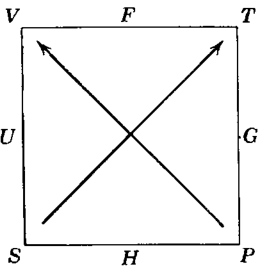
\includegraphics{fig7_1.png}
	\figcaption{热力学正方形}
	\label{fig7.1}
}

位于正方形边上的四个热力学势是它们附近的两个独立变量的函数。例如$U$是$V, S$的函数;$F$是$V, T$的函数;$G$是$T, P$的函数;等等。所有热力学势还是摩尔数$N$的函数,这在图中并未显示。

各热力学势的微分表达式中每一项的正负号由对角线箭头辅助记忆。如果箭头背离自变量,则该项是正的;而箭头指向自变量则表明该项为负。结合如下等式观察图像不难掌握这一方法:
\begin{align}
	\,\mathrm dU &= T\,\mathrm dS - P\,\mathrm dV + \sum_k \mu_k \,\mathrm dN_k \label{equ7.24} \\
	\,\mathrm dF &= -S\,\mathrm dT - P\,\mathrm dV + \sum_k \mu_k \,\mathrm dN_k \label{equ7.25} \\
	\,\mathrm dG &= -S\,\mathrm dT + V\,\mathrm dP + \sum_k \mu_k \,\mathrm dN_k  \label{equ7.26} \\
	\,\mathrm dH &= T\,\mathrm dS + V\,\mathrm dP + \sum_k \mu_k \,\mathrm dN_k  \label{equ7.27}
\end{align}

Maxwell关系可以按如下方法从图中读取。只考虑正方形顶点的量,不难看出等式的图的关系:
\begin{equation}
	\left( \frac{\partial V}{\partial S} \right)_P = \left( \frac{\partial T}{\partial P} \right)_S \quad (N_1, N_2, \dots \text{为常数})
\label{equ7.28}
\end{equation}
{
	\centering
	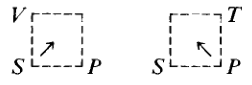
\includegraphics[scale=0.7]{equ7_28.png}
}

把图像顺时针旋转$90^\circ$, 从新图像读出:
\begin{equation}
	\left( \frac{\partial S}{\partial P} \right)_T = -\left( \frac{\partial V}{\partial T} \right)_P \quad (N_1, N_2, \dots \text{为常数})
\label{equ7.29}
\end{equation}
{
	\centering
	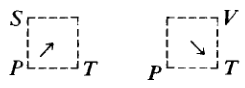
\includegraphics[scale=0.7]{equ7_29.png}
}

上图中两个箭头指向不同意味着上式有负号。再旋转图像两次可以得到其余两个Maxwell关系:
\begin{align}
	\left( \frac{\partial P}{\partial T} \right)_V &= \left( \frac{\partial S}{\partial V} \right)_T \quad (N_1, N_2, \dots, \text{为常数}) \label{equ7.30}\\
	\left( \frac{\partial T}{\partial V} \right)_S &= - \left( \frac{\partial P}{\partial S} \right)_V \quad (N_1, N_2, \dots \text{为常数}) \label{equ7.31}
\end{align}
以上四式即为最常用的Maxwell关系。

这种辅助记忆图还可以推广到变量$S, V$之外的其它变量。例如考虑经Legendre变换后的$S, N_j$, 相应的图像变为\ref{fig7.2}(a). 连接$N_j$与$\mu_j$的箭头与原图中连接$V, P$的箭头方向相反,因为$\mu_j$的地位与$-P$相同。从该图中可以读出\eqref{equ7.4}, \eqref{equ7.7}, \eqref{equ7.13}和\eqref{equ7.19}式。其它Legendre变换的辅助图类似,一般情况见\ref{fig7.2}(b).

{
	\centering
	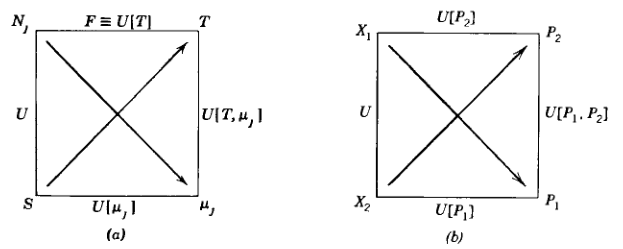
\includegraphics[scale=0.8]{fig7_2.png}
	\figcaption{}
	\label{fig7.2}
}

\subsection*{习题}


\section{单组份系统中一种导数约化的步骤}
\label{sec7.3}
在热力学的实际应用中,经常需要计算特定的偏导数以分析实验过程。例如,分析单组分系统在恒容条件下压强与温度的变化关系,显然有
\begin{equation}
	\rd T = \left( \frac{\partial T}{\partial P} \right)_{V, N} \rd P.
\label{equ7.32}
\end{equation}
然后就是要计算偏导数$(\partial T / \partial P)_{V, N}$. \ref{sec7.4}节会讨论一系列类似问题。这种偏导数量都有共同特点,求导过程中的摩尔数$N$均不变,并且同时含有广延量和强度量。{\it 所有这些导数当中只有三个是独立的,任意选定作为基的三个量之后,其余的偏导数都可以用这三者表示。} 通常选择$c_P, \alpha, \kappa_T$作为基。

$c_P, \alpha, \kappa_T$意味着使用Gibbs表象,因为在该表象下三个量可以用$\partial^2 g / \partial T^2, \partial^2 g / \partial T \partial P$以及$\partial^2 g / \partial P^2$简单表述:它们分别等于$-c_P / T, v\alpha$以及$-v \kappa_T$. 在系统摩尔数不变的情况下,其余的二阶导数都依赖于它们。

{\it 所有一阶导数(既包括对广延量、也包括对强度量求导)可以表为Gibbs势二阶偏导数量的函数,例如上面的$c_P, \alpha, \kappa_T$就构成一组完备集(在摩尔数不变的情况下)。}

“导数约化”的过程原则上十分直接,只需要把熵$S$替换成$-\partial G / \partial T$, $V$换成$\partial G / \partial P$,接着原始偏导数量用$G$对$T, P$的二阶混合导数表示出来即可。但实际上这么干会相当复杂。

学过热力学的人的一个基本技能是熟练掌握“导数约化”技术——将任意偏导数量用已知的偏导数基表示。为此,我们提出一种基于上一节“正方形记忆图”的方法,并且整理成了按部就班的套路。只有进行大量练习才能真正掌握。

以下假设求导过程的摩尔数均不变。要将给定的导数表示为$c_P, \alpha, \kappa_T$的函数。之后会用到如下微分恒等式(见附录A):
\begin{equation}
	\left( \frac{\partial X}{\partial Y} \right)_Z = 1 \Big/ \left(\frac{\partial Y}{\partial X} \right)_Z 
\label{equ7.33}
\end{equation}
以及
\begin{align}
	\left( \frac{\partial X}{\partial Y} \right)_Z &= \left( \frac{\partial X}{\partial W} \right)_Z \Bigg/ \left( \frac{\partial Y}{\partial W} \right)_Z \label{equ7.34} \\
	\left( \frac{\partial X}{\partial Y} \right)_Z &= - \left( \frac{\partial Z}{\partial Y} \right)_X \Bigg/ \left( \frac{\partial Z}{\partial X} \right)_Y \label{equ7.35}
\end{align}

接着,按照顺序执行下列运算:

\begin{enumerate}
\item {\bf 如果导数中含有势函数,那么把它们化到分子中,并且利用热力学正方形包含的等量关系(\eqref{equ7.24} - \eqref{equ7.27}式)将它消去。}
\paragraph{例} 化简导数$(\partial P / \partial U)_{G, N}$.
\begin{align}
	\left( \frac{\partial P}{\partial U} \right)_{G, N} &= \left[ \left( \frac{\partial U}{\partial P} \right)_{G, N} \right]^{-1} \tag{by \eqref{equ7.33} } \\
	&= \left[ T \left( \frac{\partial S}{\partial P} \right)_{G, N} - P \left( \frac{\partial V}{\partial P} \right)_{G, N} \right]^{-1} \tag{by \eqref{equ7.34} }  \\
	&= \left[ -T \left( \frac{\partial G}{\partial P} \right)_{S, N} \Bigg/ \left( \frac{\partial G}{\partial S} \right)_{P, N} + P \left( \frac{\partial G}{\partial P} \right)_{V, N} \Bigg/ \left( \frac{\partial G}{\partial V} \right)_{P, N} \right]^{-1} \tag{by \eqref{equ7.35} } \\
	&= \left[ -T \frac{-S (\partial T / \partial P)_{S, N} + V}{-S (\partial T / \partial S)_{P, N}} + P \frac{-S(\partial T / \partial P)_{V, N} + V}{-S (\partial T / \partial V)_{P, N}} \right]^{-1} \tag{by \eqref{equ7.26} }
\end{align}
经过处理后的表达式不含任何势函数,只含有导数。然后按如下步骤处理导数量。
\item {\bf 如果导数中含有化学势,那么把它化到分子中,再利用Gibbs-Duhem关系}$\rd \mu = -s \,\rd T + v\,\rd P${\it 消去它。}

\paragraph{例} 化简$( \partial \mu / \partial V)_{S, N}$.

\[
	\left( \frac{\partial \mu}{\partial V} \right)_{S, N} = -s \left( \frac{\partial T}{\partial V} \right)_{S, N} + v \left( \frac{\partial P}{\partial V} \right)_{S, N}
\]
\item {\bf 如果导数中含有熵,则将它化到分子。如果正方形记忆图中的四个Maxwell关系可以消去这个熵的导数,则调用它消去。如果Maxwell关系不能消去熵,那么利用\eqref{equ7.34}式(令其中的$w = T$)凑出$\partial S / \partial T$, 这样分子就能表示为热容$c_v$或$c_P$的函数。}

\paragraph{例} 考虑第1步出现的导数$(\partial T / \partial P)_{S, N}$:
\begin{align}
	\left( \frac{\partial T}{\partial P} \right)_{S, N} &= - \left( \frac{\partial S}{\partial P} \right)_{T, N} \Bigg/ \left( \frac{\partial S}{\partial T} \right)_{P, N} \tag{by \eqref{equ7.35}} \\
	&= \left( \frac{\partial V}{\partial T} \right)_{P, N} \Bigg/ \frac{N}{T} c_P \tag{by \eqref{equ7.29}}
\end{align}

\paragraph{例} 考虑导数$(\partial S / \partial V)_{P, N}$, 利用Maxwell关系$(\partial S / \partial V)_{P, N} = (\partial P / \partial T)_{S, N}$ (\eqref{equ7.28}式)不能消去熵,因此不调用Maxwell关系,而是凑出$\partial S / \partial T$:
\begin{equation}
	\left( \frac{\partial S}{\partial V} \right)_{P, N} = \frac{(\partial S / \partial T)_{P, N}}{(\partial V / \partial T)_{P, N}} = \frac{(N / T) c_P}{(\partial V / \partial T)_{P, N}} \tag{by \eqref{equ7.34}}
\end{equation}
于是将导数化成了不含势函数也不含有熵的形式,只包括$V, P, T$(当然还有$N$)。
\item {\bf 将$V$化入分子,这样出现的量都能表示为$\alpha$与$\kappa_T$的函数。}

\paragraph{例} \begin{equation}
	\left( \frac{\partial T}{\partial P} \right)_{V, N} = -\left( \frac{\partial V}{\partial P} \right)_{T, N} \Bigg/ \left( \frac{\partial V}{\partial T} \right)_{P, N} = \frac{\kappa_T}{\alpha} \tag{by \eqref{equ7.35}}
\end{equation}

\item {\bf 最初给定的导数经以上步骤已经化成了用$c_v, c_P, \alpha, \kappa_T$表示的形式。恒容热容可以用下式消去:}
\begin{equation}
	c_v = c_P - \frac{Tv\alpha^2}{\kappa_T}
\label{equ7.36}
\end{equation}
\end{enumerate}

上式即\eqref{equ3.75}式的变形,它经常被用到,应该牢记。读者也要掌握上式的推导(见习题7.3-2)。

上面导数约化的步骤以单组分系统为例,但也可以推广到多组分系统,只要组分的化学势$\mu_j$不出现在导数中(因为单组分系统的化学势是通过Gibbs-Duhem关系消去的,对于多组分系统而言G-D关系将一种化学势化为了其他化学势)。

\subsection*{习题}

\section{简单应用}
\label{sec7.4}
本节介绍\ref{sec7.3}节的几个代表性应用,每个例子以一个问题 —— 研究某一参量在其他参量变化的情况下的变化情况 —— 开始。最简单的情形是简单系统在恒容条件下,温度变化$\Delta T$对应的压强变化$\Delta P$.

我们用两种方法解决该问题。首先,如果基本方程已知,则可以直接求解。第二种方法的条件是已知$c_P, \alpha, \kappa_T$,且各参量的变化为小量。

\subsection*{绝热压缩}
考虑被绝热壁包围的单组分简单系统(粒子数为$N$)。系统的初始温度与压强已知,经准静态压缩后,压强从$P_i$变为$P_f$. 如何得出其他热力学量(如体积、温度、内能、化学势)的变化?

求解的关键在于——绝热壁表明了系统的熵在准静态过程中不变。该判断的依据当然是准静态过程中$\dbar Q = T \rd S$.

以温度为例,计算其变化。首先假设系统的基本方程已知,对它微分可得两个状态方程$T = T(S, V, N)$与$P = P(S, V, N)$. 初始温度与压强已知,于是可得初始体积与熵。联立上两个状态方程消去$V$得到温度$T$关于$S, P, N$的关系式,于是得到温度的变化:
\begin{equation}
	\Delta T = T(S, P_f, N) - T(S, P_i, N)
\label{equ7.37}
\end{equation}

如果基本方程未知,但知道$c_P, \alpha, \kappa_T$,并且压强的变化是小量,则有
\begin{equation}
	\rd T = \left( \frac{\partial T}{\partial P} \right)_{S, N} \rd P 
\label{equ7.38}
\end{equation}
利用\ref{sec7.3}节介绍的套路可以算出
\begin{equation}
	\rd T = \frac{Tv\alpha}{c_P} \rd P 
\label{equ7.39}
\end{equation}

化学势的求解过程相似。答案是(仍然要求压强变化量是小量):
\begin{align}
	\rd \mu &= \left( \frac{\partial \mu}{\partial P} \right)_{S, N} \rd P \label{equ7.40} \\
	&= \left( v - \frac{sTv\alpha}{c_P} \right) \rd P \label{equ7.41}
\end{align}

系统在(无穷小)绝热压缩过程中体积的相对变化由{\it 绝热压缩率}$\kappa_S$表征,定义见$\eqref{equ3.73}$式。那里曾提到过$\kappa_S$可以由$\kappa_T, c_P, \alpha$表示(\eqref{equ3.76}式,又见习题3.9-5),这里建议读者完成习题7.4-8。

\subsection*{等温压缩}
系统在恒温、摩尔数不变的条件下准静态压缩,压强从$P_i$变到$P_f$. 还是要计算$U, S, V, \mu$的变化。通过对基本方程与状态方程一通捣鼓以消去变量,可以得到$U, S, V, \mu$各自关于$T, P, N$的表达式,于是可得各参量的变化。

对于压强的微小变化,有
\begin{align}
	\rd S &= \left( \frac{\partial S}{\partial P} \right)_{T, N} \rd P \label{equ7.42} \\
	&= -\alpha V \rd P \label{equ7.43}
\end{align}
同样也有
\begin{align}
	\rd U &= \left( \frac{\partial U}{\partial P} \right)_{T, N} \rd P \label{equ7.44} \\
	&= ( -T \alpha V + PV \kappa_T) \,\rd P \label{equ7.45}
\end{align}
其他参量同理。

有时需要求出为保持系统在压缩过程保持温度不变而从系统吸收的热量。首先还是假设基本方程已知,于是热量变化为
\begin{equation}
	\Delta Q = T\Delta S = TS(T, P_f, N) - TS(T, P_i, N)
\label{equ7.46}
\end{equation}
其中基本方程$S(U, V, N)$(通过与状态方程联立等等一通折腾)变成了$S(T, P, N)$的形式。 

如果不知道基本方程:首先考虑无穷小的等温压缩过程,由\eqref{equ7.43}式可得
\begin{equation}
	\dbar Q = -T\alpha V \,\rd P 
\label{equ7.47}
\end{equation}
然后是有限大(非无穷小)的等温压缩。注意,基本方程未知,\eqref{equ7.46}式不能用。如果已知$\alpha, V$关于$T, P$的函数,那么对\eqref{equ7.47}式沿等温过程积分就得到热量变化:
\begin{equation}
	\Delta Q = -T \int_{P_i}^{P_f} \alpha V \,\rd P 
\label{equ7.48}
\end{equation}
这个解必然与\eqref{equ7.46}式一致。

\subsection*{自由膨胀}
第三个例子是自由膨胀过程(习题3.4-8, 4.2-3接触过它)。系统的初始体积为$V_i$,突然释放使系统膨胀到体积$V_f$. 如果是气体系统(当然,下面的推导不只针对气体),则该过程可以用如下装置方便地实现:某一刚性容器由隔板分为两部分,一部分是气体,另一部分真空。突然撤去隔板,则气体自发膨胀充满整个容器。系统的其他参量在该过程的变化如何求解?

既然是自由膨胀,则系统的内能不变。系统既未向外传热,也没有对外做功。

如果已知温度关于$U, V, N$的表达式,则有
\begin{equation}
	T_f - T_i = T(U, V_f, N) - T(U, V_i, N)
\label{equ7.49}
\end{equation}
如果体积的变化为小量,则
\begin{align}
	\rd T &= \left( \frac{\partial T}{\partial V} \right)_{U, N} \rd V \label{equ7.50} \\
	&= \left( \frac{P}{N c_v} - \frac{T\alpha}{N c_v \kappa_T} \right) \rd V \label{equ7.51}
\end{align}

与前两例不同,自由膨胀过程本质上既不可逆,也不是准静态的(见习题4.2-3)。
\begin{example}
三次元的真实过程不可能像例子们那样简洁可爱,没有任何参量在演化前后是不变的。例如计算发动机气缸在膨胀冲程(expansion stroke,又称为做功冲程)前后的温度变化,气缸壁可以自由传热,故而该膨胀过程既不等温也不绝热。然而,经验表明温度可以近似表为体积的函数,于是该过程可以用$T = T(V)$定义。读者会遇到许多将真实过程模型化的情况,这个例子可以作为参考。

某一单组分系统(摩尔数$N$)经膨胀过程,体积从$V_1$变为$V_2$,温度从$T_1$降至$T_2$,并且观测到温度随体积线性减少。计算在膨胀过程中外界对系统做的功以及传入系统的热量,答案用$c_P, \alpha, \kappa_T$的表达式或积分表示。

{\bf 求解:}\\
首先注意到函数$c_P (T, P), \alpha(T, P), \kappa_T (T, P)$, 以及$v(T, P)$ (它们可以查表求出)是有冗余的。\ref{sec3.9}的例题已经推导过,从前三个函数可以导出最后一个。

题目里的膨胀过程在$T\text{-}V$图上对应的轨迹为
\begin{align*}
	T &= A + BV; \\
	A &= \frac{T_1 V_2 - T_2 V_1}{V_2 - V_1}; \\
	B &= \frac{T_2 - T_2}{V_2 - V_1}.
\end{align*}
此外,$v(T, P)$可以转化为$P$关于$T, v$的函数,于是轨迹上每一点的压强是已知的,将上式$T$关于$v$的关系代入即可得$P$关于$v$的关系: 
\[
	P = P(T, V) = P(A + BV, V)
\]
于是得到在膨胀过程中,外界对系统做的功:
\[
	W = \int_{V_1}^{V_2} P(A + BV, V) \rd V 
\]
这个积分只有数值解,不过用计算器能够算出来。\sout{因此考试也会考} 

为了计算传入系统的热量,考虑$S$关于$T, V$的函数, 
\begin{align*}
	\rd S &= \left( \frac{\partial S}{\partial T} \right)_V \rd T + \left( \frac{\partial S}{\partial V} \right)_T \rd V \\
	&= \frac{N}{T} c_v \rd T + \left( \frac{\partial P}{\partial T} \right)_V \rd V \\
	&= \left( \frac{Nc_P}{T} - \frac{V \alpha^2}{\kappa_T} \right) \rd T + \frac{\alpha}{\kappa_T} \rd V 
\end{align*}
在膨胀过程的轨迹上有$\rd T = B \rd V$,于是 
\[
	\rd S = \left( NB\frac{c_P}{T} - \frac{BV\alpha^2}{\kappa_T} + \frac{\alpha}{\kappa_T} \right) \rd V 
\]
传热量为
\[
	Q = \int_{V_1}^{V_2} \Big[ NBc_P - (A + BV)(BV\alpha - 1)\alpha / \kappa_T \Big] \rd V 
\]
这个积分还是只能利用轨迹上不同的$V$对应的$P, T$的值解出数值解。

有时为了方便,可以把一定范围内的数据用多项式拟合得到近似的表达式;许多程序都能进行拟合,这样积分既可以用数值法,又可以通过“解析法”计算出来。
\end{example}

\begin{example}
 某种物质在$P-v$图上的两个状态$A, D$定义为
\begin{align*}
	P_A &= \SI{1e5}{Pa} \quad v_A = \SI{2e-2}{m^3 \per mole} \\
	P_D &= \SI{1e4}{Pa} \quad v_D = \SI{1e-1}{m^3 \per mole}
\end{align*}

此外$T_A = \SI{350.0}{K}$. 设1摩尔该物质初态为$A$, 可逆热源为$\SI{150}{K}$的热库,主系统从状态$A$演化到$D$,最多能够传给可逆功源多少功?

其他已知条件有,系统的绝热线为
\[
	Pv^2 = \text{constant} \quad (s = \text{constant})
\]
$\SI{1e5}{Pa}$下的$c_P, \alpha$为 
\begin{align*}
	c_P &= Bv^{2/3} \quad ( P = \SI{1e5}{Pa}); \\
	B &= 10^{8/3} = \SI{464.2}{J \per m^2.K} \\
	\alpha &= 3/T \quad ( P = \SI{1e5}{Pa})
\end{align*}
$\kappa_T$未知。

读者在看下面的答案之前一定要自己分析一下题目。

{\bf 求解:}\\
为求解从$A \to D$的可逆过程对应的最大功,需要求出$u_D - u_A$以及$s_D - s_A$. 

经过状态$D$的绝热线方程为$Pv^2 = \SI{1e2}{Pa.m^6}$; 它与$P = \SI{1e5}{Pa}$等压线相交于点$C$:
\[
	P_C = \SI{1e5}{Pa}, \quad v_c = 10^{-3/2}\, \mathrm{m}^3 = \SI{3.16e-2}{m^3}.
\]
于是可以从$A$经过两步演化到$D$状态,首先是$A \stackrel{\text{等压过程}}{\longrightarrow}$,然后$C \stackrel{\text{等熵(绝热)过程}}{\longrightarrow} D$。计算这两个过程的$u_C - u_A$、$s_C - s_A$以及$u_D - u_C$、$s_D - s_C$,最终得到$u_D - u_A$、$s_D - s_A$.

首先考虑从$A$到$C$的等压过程:
\[
	\rd u = T \rd s - P \rd v = \left( \frac{c_P}{v\alpha} - P \right) \rd v = \left( \frac{1}{3} B v^{-1/3} T - P_A \right) \rd v
\]
由于不知道等压过程中的$T(v)$关系,因此上式不能直接积分。为计算等压过程的$T(v)$,首先有
\[
	\left( \frac{\partial T}{\partial v} \right)_P = \frac{1}{v \alpha} = \frac{T}{3v} \quad (\text{for}\ P = P_A)
\]
积分得
\[
	\ln \left( \frac{T}{T_A} \right) = \frac{1}{3} \ln \left( \frac{v}{v_A} \right)
\]
于是可得 
\[
	T = 350.9 \times (50v)^{1/3} \quad (\text{等压过程}P = \SI{1e5}{Pa})
\]

接着计算$u_C - u_A$:
\[
	\rd u = \left[ \frac{1}{3} B \times 350.9 \times (50)^{1/3} - 10^5 \right] \rd v \approx 10^5 \rd v
\]
于是 
\[
	u_C - u_A = 10^5 \times (v_C - v_A) = \SI{1.16e3}{J}
\]

下面计算$u_D - u_C$. 从$C$到$D$为绝热过程,
\[
\begin{split}
	u_D - u_C &= -\int_{v_C}^{v_D} P\rd v = -10^2 \int_{v_C}^{v_D} \frac{\rd v}{v^2} \\
	&= 10^2 [v_D^{-1} - v_C^{-1} ] = -\SI{2.16e3}{J}
\end{split}
\]
最终得到了内能之差
\[
	u_D - u_A = -\SI{1e3}{J}
\]

接着考虑熵差$s_D - s_A = s_C - s_A$. 在等压线$AC$上:
\[
	\rd s = \left( \frac{\partial s}{\partial v} \right)_P \rd v = \frac{c_P}{Tv\alpha} \rd v = \frac{1}{3} B v^{-1/3} \rd v
\]
于是 
\[
	s_D - s_A = s_C - s_A = \frac{1}{2} B \left[v_C^{2/3} - v_A^{2/3} \right] = \SI{6.1}{J \per K}
\]
求出整个过程的$\Delta u$与$\Delta s$之后,余下的最大功问题就好办了。主系统熵的增量对应于从热库中{\it 吸收的}热量:
\[
	(-Q_{\text{热库}}) = T_{\text{热库}} \Delta s = 150 \times 6.1 = \SI{916}{J}
\]
传给可逆功源的总能量为$(-\Delta u) + (-Q_{\text{热库}})$,也就是 
\[
	\text{传递的功} = \SI{1.92e3}{J}
\]

\end{example}


\subsection*{\sout{二十多道}习题}



\section{推广:以磁系统为例}
\label{sec7.5}
对于简单系统以外的其他系统可以建立一套相似的Legendre变换体系、Maxwell关系、辅助记忆图以及导数约化方法。

以磁系统为例,它的基本方程为(见\ref{sec3.8}节和附录B):
\begin{equation}
	U = U(S, V, I, N)
\label{equ7.52}
\end{equation}
可以对$S, V, N$做Legendre变换(磁矩$I$视为寻常参量)。例如系统的焓是$S, P, I, N$的函数:
\begin{equation}
	H \equiv U[P] = U + PV = H(S, P, I, N)
\label{equ7.53}
\end{equation}
当然也可以类比着对磁场量进行Legendre变换:
\begin{equation}
	U[B_e] = U - B_e I 
\label{equ7.54}
\end{equation}
变换得到的势是$S, V, B_e, N$的函数,系统的在外磁场恒定下的平衡条件为这个势取最小值。

其他各种Legendre变换的结果在图\ref{fig7.3}中。左边的Maxwell关系式可以从右边的图中按照之前的套路读出。

{
	\centering
	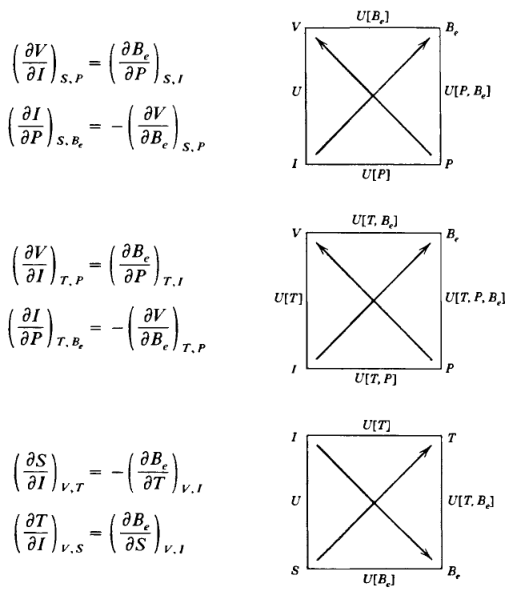
\includegraphics[width=\textwidth]{fig7_3.png}
	\figcaption{}
	\label{fig7.3}
}

“磁焓”$U[P, B_e] \equiv U + PV - B_e I$是有趣又有用的势函数。在压强、外磁场恒定的条件下,系统的磁焓取最小值。此外,根据\eqref{equ6.29}式的磁焓变体,$\rd U[P, B_e] = T\rd S = \dbar Q$($P, B_e, N$不变)。由此可见磁焓$U[P, B_e]$在压强、外磁场恒定的情况下就像系统的“热量势(potential for heat)”那样。

\begin{example}
某系统的基本方程与“顺磁模型”相同(\eqref{equ3.66}式),$T_0 = \SI{200}{K}, I_0^2 / 2R = \SI{10}{Tesla^2.K\per m^2.J}$。系统的摩尔数为$2$,在$B_e = \SI{0.2}{Tesla}$($\SI{2000}{gauss}$)的外磁场下保持压强恒定,从初始温度$\SI{5}{K}$加热到$\SI{10}{K}$. 求传入系统的能量。

{\bf 求解:}\\
传入系统的能量正是“磁焓”$U[P, B_e]$的改变量。顺磁模型的基本方程与体积无关,$P \equiv \partial U / \partial V = 0$, 于是$U[P, B_e]$退化到$U - B_e I = U[B_e]$. 再根据\eqref{equ3.66}式,$U = NRT, I = (NI_0^2 / 2RT) B_e$, 于是$U[P, B_e] = U[B_e] = NRT - (NI_0^2 / 2RT) B_e^2$. 因此 
\begin{align*}
	Q &= N \left[ R\Delta T - \frac{I_0^2}{2R} B_e^2 \Delta \left( \frac{1}{T} \right) \right] \\
	&= 2 [8314 \times 5 + 10 \times 0.04 \times 0.1] \,\mathrm{J} = \SI{83.15}{J}
\end{align*}

注意第二项的磁过程对传热的贡献相对于非磁过程(第一项)来说很小;实际中非磁过程对固体热容的贡献在低温下急剧降低,以至于比磁部分小。不妨回顾习题3.9-6.

\end{example}


\subsection*{习题}
